%Dies ist die Hauptseite des Dokumentes. Es werden u. a. alle Kapitel,
%Einstellung im Header eingebunden.  Veränderungen müssen in folgenden Dateien
%vorgenommen werden:
      %- config.tex
      %- einzelne Kapitel (evtl. erweitern)

%Hier sind alle Einstellungen enthalten, die sich auf das Seiten- und
%Dokumentenlayout beziehen

\documentclass[
  11pt,                   % Schriftgröße
  DIV12,
  german,                 % für Umlaute, Silbentrennung etc.
  oneside,                % einseitiges Dokument
  titlepage,              % es wird eine Titelseite verwendet
  parskip=half,           % Abstand zwischen Absätzen (halbe Zeile)
  headings=normal,        % Größe der Überschriften verkleinern
  captions=tableheading,  % Beschriftung von Tabellen unterhalb ausgeben
  final                   % Status des Dokuments (final/draft)
]{scrreprt}               %


%------Ändern von Schriftschnitten - (Muss ganz am Anfang stehen !) ------------
\usepackage{fix-cm}


%------Umlaute -----------------------------------------------------------------
%   Umlaute/Sonderzeichen wie äüöß können direkt im Quelltext verwenden werden.
%    Erlaubt automatische Trennung von Worten mit Umlauten.
\usepackage[T1]{fontenc}
\usepackage[utf8]{inputenc}

%------Anpassung der Landessprache----------------------------------------------
\usepackage[ngerman]{babel}

%------Einfache Definition der Zeilenabstände und Seitenränder------------------
\usepackage{geometry}
\usepackage{setspace}

%------Schriftgrößenanpassung von einzelnen Textpassagen------------------------
\usepackage{relsize}

%------Trennlinien in Kopf- und Fusszeile
\usepackage[headsepline, footsepline, ilines]{scrlayer-scrpage}

%------Grafiken und Farben -----------------------------------------------------
\usepackage{graphicx}

%------Packet zum Sperren, Unterstreichen und Hervorheben von Texten------------
\usepackage{soul}

%------ergänzende Schriftart----------------------------------------------------
\usepackage{helvet}

%------Lange Tabellen-----------------------------------------------------------
\usepackage{longtable}
\usepackage{array}
\usepackage{ragged2e}
\usepackage{lscape}
\usepackage{tabularx}

%------DocTeX-------------------------------------------------------------------
\usepackage{changepage}
\usepackage{scalerel}
\newcolumntype{R}{>{\raggedright\arraybackslash}X}%

%------PDF-Optionen-------------------------------------------------------------
\usepackage[
  bookmarks,
  bookmarksopen=true,
  colorlinks=true,
  linkcolor=black,        % einfache interne Verknüpfungen
  anchorcolor=black,      % Ankertext
  citecolor=black,        % Verweise auf Literaturverzeichniseinträge im Text
  filecolor=black,        % Verknüpfungen, die lokale Dateien öffnen
  menucolor=black,        % Acrobat-Menüpunkte
  urlcolor=black,         % Farbe für URL-Links
  backref,                % Zurücktext nach jedem Bibliografie-Eintrag als
                          % Liste von Überschriftsnummern
  pagebackref,            % Zurücktext nach jedem Bibliografie-Eintrag als
                          % Liste von Seitenzahlen
  plainpages=false,       % zur korrekten Erstellung der Bookmarks
  pdfpagelabels,          % zur korrekten Erstellung der Bookmarks
  hypertexnames=false,
  colorlinks=true,   % zur korrekten Erstellung der Bookmarks
  linktocpage             % Seitenzahlen anstatt Text im Inhaltsverzeichnis verlinken
  ]{hyperref}
  \hypersetup{
    colorlinks=true, %set true if you want colored links
    linktoc=all,     %set to all if you want both sections and subsections linked
  }
  \usepackage{verbatim}
  \usepackage{lipsum}                     % Dummytext
  \usepackage{xargs}                      % Use more than one optional parameter in a new commands
  \usepackage[pdftex,dvipsnames]{xcolor}  % Coloured text etc.

  \usepackage[colorinlistoftodos,prependcaption,textsize=tiny]{todonotes}

%------Glossar------------------------------------------------------------------
\usepackage[translate=babel,toc]{glossaries}
      % enthält eingebundene Packete

%------Seitenränder-------------------------------------------------------------
\geometry{verbose,                     % zeigt die eingestellten Parameter beim
                                       % Latexlauf an
      paper=a4paper,                   % Papierformat
      top=25mm,                        % Rand oben
      left=25mm,                       % Rand links
      right=25mm,                      % Rand rechts
      bottom=45mm,                     % Rand unten
      pdftex                           % schreibt das Papierformat in die
                                       % Ausgabe damit Ausgabeprogramm
                                       % Papiergröße erkennt
  }

%Seitenlayout
\onehalfspace        % 1,5-facher Abstand

%------Kopf- und Fußzeilen -----------------------------------------------------
\pagestyle{scrheadings}

%------Kopf- und Fußzeile auch auf Kapitelanfangsseiten ------------------------
\renewcommand*{\chapterpagestyle}{scrheadings}

%------Schriftform der Kopfzeile -----------------------------------------------
\renewcommand{\headfont}{\normalfont}

%----Spezielle Befehle
\newcommand{\lfk}[1]{$\langle LF#1\rangle$}

%----Farben
\definecolor{tubsRed}{cmyk}{0.1,1.0,0.8,0.0}
\definecolor{tuRed}{cmyk}{1.0,0.0,0.6,0.0}

%------Kopfzeile----------------------------------------------------------------
\setheadsepline{1pt}[\color{tuRed}]
\setlength{\headheight}{21mm}        % Höhe der Kopfzeile
\ihead{\large{\textsc{\praktikumTitel}}\\    % Text in der linken Box
       \small{\projektTitel}}
\chead{}                            % Text in der mittleren Box

%----Fusszeile
\setfootsepline{1pt}[\color{tuRed}]
\cfoot{}                            % Text in mittlerer Box
\ofoot{\pagemark}                    % Seitenzahl in rechter Box



%------Labels mit eigenem Text für \ref ----------------------------------------
\makeatletter
\def\namedlabel#1#2{\begingroup
#2%
\def\@currentlabel{#2}%
\phantomsection\label{#1}\endgroup
}
\makeatother


%------Neue Environments -------------------------------------------------------

\newcommand{\refsetcounter}[2]{\setcounter{#1}{#2}\addtocounter{#1}{-1}\refstepcounter{#1}}

%Funktion im Pflichtenheft
\newcounter{functioncount} 
\newenvironment{function}[2]{\refsetcounter{functioncount}{#1}\large\textbf{\sffamily{#2 }}\namedlabel{F#1}{$\langle F#1\rangle$}\normalsize\begin{description}\setlength{\itemsep}{-5pt}}{\end{description}}

%Daten im Pflichtenheft
\newcounter{datacount}
\newenvironment{data}[2]{\refsetcounter{datacount}{#1}\textbf{#2} \namedlabel{D#1}{$\langle D#1\rangle$}\\}{}

%Kriterien im Pflichtenheft
\newcounter{mustcount} 
\newcommand{\must}[2]{\refsetcounter{mustcount}{#1}\namedlabel{RM#1}{$\langle RM#1\rangle$} #2\\}

\newcounter{wishcount}
\newcommand{\wish}[2]{\refsetcounter{wishcount}{#1}\namedlabel{RW#1}{$\langle RW#1\rangle$} #2\\}

\newcounter{notfunctional}
\newcommand{\notfunctional}[2]{\refsetcounter{notfunctional}{#1}\namedlabel{NF#1}{$\langle NF#1\rangle$} #2\\}

\newcommand{\wont}[2]{\refsetcounter{datacount}{#1}\namedlabel{RN#1}{$\langle RN#1\rangle$} #2\\}

%Qualitätsanforderungen im Pflichtenheft
\newcommand{\qualityReq}[2]{\refsetcounter{datacount}{#1}\namedlabel{Q#1}{$\langle Q#1\rangle$} #2\\}

% Benutzeroberflächen im Pflichtenheft
\newcounter{uicount}
\newenvironment{ui}[2]{\refsetcounter{uicount}{#1}\textbf{#2} \namedlabel{UI#1}{$\langle UI#1\rangle$}\\}{}

% Klassen
\newcounter{classcount}
\newenvironment{class}[2]{\refsetcounter{classcount}{#1}\textbf{#2}\namedlabel{CL#1}{$\langle CL#1\rangle$}\begin{description}\setlength{\itemsep}{-5pt}}{\end{description}}

% Entitäten
\newcounter{entitycount}
\newenvironment{entity}[2]{\refsetcounter{entitycount}{#1}\textbf{#2} \namedlabel{E#1}{$\langle E#1\rangle$}\\}{}

% Component
\newcounter{componentcount}
\newenvironment{component}[2]{\refsetcounter{componentcount}{#1}\textbf{Komponente \namedlabel{C#1}{$\langle C#1\rangle$}: #2}\\}{}

% Interface
\newcounter{interfacecount}
\newenvironment{interface}[2]{\refsetcounter{interfacecount}{#1}\textbf{Schnittstelle \namedlabel{I#1}{$\langle I#1\rangle$}: #2}\\}{}

% Testfall
\newcounter{testcasecount}
\newenvironment{testcase}[2]{\refsetcounter{testcasecount}{#1}\textbf{Testfall #2}\namedlabel{T#1}{$\langle T#1\rangle$}\normalsize\begin{description}\setlength{\itemsep}{-5pt}}{\end{description}\hspace{7.5em}}
           % Diese Datei enthält alle
                                           % Layouteinstellungen
\newcommand{\dokumentTitel}{Entwurfsheft}
% Definition von globalen Parametern, die derzeit auf der Titelseite und in der
% Kopfzeile verwendet werden. Der in <> gesetzte Text ist zu verändern.

\newcommand{\praktikumTitel}{Praxis der Softwareentwicklung}
\newcommand{\projektTitel}{Solidarische Raumnutzung}

\newcommand{\semester}{Wintersemester 2024/25}
\newcommand{\institut}{
	Institut für Anthropomatik und Robotik (IAR)\\
	Forschungsgruppe Mensch-Maschine-Interaktion und Barrierefreiheit (MBI)\\
	Prof. Dr. Kathrin Gerling\\
	Adenauerring 10, Gebäude 50.28\\
	76131 Karlsruhe\\
}
\newcommand{\institutsLogo}{common/hci.png}
\newcommand{\kitlogo}{common/kit_logo.jpg}
\newcommand{\betreuer}{Sabrina Burtscher}


\makeglossaries

%------Beginn des Gesamtdokumentes----------------------------------------------
\begin{document}

%------Eingebundene Seiten, Verzeichnisse bzw. Kapitel--------------------------
% Dies ist die Titelseite.
% Die Ausgabe darf 1 Seite nicht überschreiten, also ggf. Abstände anpassen
% Die Angabe in [...] gibt den Abstand nach der entsprechenden Zeile an.


%----Stil dieser Seite----------------------------------------------------------
\thispagestyle{plain}      % Kopfzeile bleibt leer

%----Beginn der Titelseite------------------------------------------------------
\begin{titlepage}

\vspace*{-3.8cm}
\hspace*{-2cm}\begin{minipage}{1.25\textwidth}

\includegraphics[width=5.3cm]{common/kit_logo}\setlength{\unitlength}{1mm}\begin{picture}(00,00)(-10,0)\color{tuRed}\put(000,004){\line(1,0){140}}\end{picture}%\hfill
\parbox[b]{0.68\textwidth}{\hfill\includegraphics[width=8cm,height=2.4cm,keepaspectratio]{\institutsLogo}\\~}
\end{minipage}


~\\[5ex]

%----zentrierte Ausrichtung über die gesamte Seite----------------------------
\begin{center}

%----Titel des Praktikum (\praktikumTitel in newComments zu verändern)--------
{\relsize{4}{\textbf{\textsc{\praktikumTitel}}}}\\[5ex]

%----Titel des Teilprojektes (\projektTitel in newComments verändern)---------
{\relsize{3}{\textbf{\textsc{\projektTitel}}}}\\[5ex]

Praxis der Softwareentwicklung (PSE)\\
\semester\\[6ex]

{\relsize{3}{\textbf{\dokumentTitel}}}\\[5ex]

%----Daten des Auftraggebers
Karlsruher Institut für Technologie (KIT)\\
\institut[2ex]
\textbf{Betreuer: \betreuer}\\[5ex]

\textbf{Projektteilnehmer:}\\

% ----Tabelle der Praktikumsteilnehmer------------------------------------------
\begin{tabular}{l<{\hspace{20mm}} l<{\hspace{30mm}}}\\
  Name                   &   E-Mail-Adresse\\      % Zeilenüberschift

  \hline                    % Linie unterhalb der Zeilenüberschrift

  %----Nachfolgend alle Namen und E-Mail-Adressen der Teilnehmer einfügen
  Antonia Ammon  &  <E-Mail-Adresse>\\
  Ben Steinle &  <E-Mail-Adresse>\\
  Johannes Frohnmeyer &  <E-Mail-Adresse>\\
  Alexander Klee &  <E-Mail-Adresse>\\
  Jannik Hönlinger &  <E-Mail-Adresse>\\

\end{tabular}

%Zur Vereinheitlichung sollten hier die TU Braunschweig Emailadressen benutzt werden. % enthält Tabelle der Praktikumsteilnehmer

\vfill
Karlsruhe, \today

\end{center}
\end{titlepage}
                       % Titelseite

%!TEX root = ../Pflichtenheft.tex

\chapter{Glossar}

\begin{description}
\item[CI/CD] Baut automatisiert Software, führt Tests durch und veröffentlicht Artefakte
\item[Docker] Software zur Bereitstellung von Anwendungen innerhalb von Containern
\item[Container] Isolierte Umgebung um Software unabhängig von der zugrunde liegenden Umgebung auszuführen
\item[Browser] Software zum Navigieren von Webseiten, zum Beispiel Firefox oder Chrome
\item[Git] Software zur Versionsverwaltung von Softwareprojekten
\item[GitHub] Plattform zur Versionsverwaltung von Softwareprojekten, nutzt Git
\item[IDE] (Integrated Development Environment) Software, welche alle Werkzeuge zur Softwareentwicklung in einem Programm kombiniert
\item[AMD64] Verbreitete Prozessorarchitektur von Intel und AMD
\item[RAM] (Random Access Memory) Arbeitsspeicher
\item[VM] (Virtuelle Maschine) Software zur Simulation eines Computers
\item[PostgreSQL] Objekt-Relationales Datenbankmanagementsystem, welches zum Speichern und Verwalten von Daten verwendet wird
\item[HTML] (Hypertext Markup Language) Eine Sprache um die Struktur und den Inhalt einer Website zu definieren
\item[CSS] Cascading Style Sheets, ist eine Sprache um das Visuelle aussehen einer Website zu definieren
\item[JavaScript] Programmiersprache um das Logische verhalten von Webseiten zu steuern
\item[SSR] (Server-Side Rendering) Methode um das HTML einer Website auf dem Server zu produzieren, anstelle des Browsers
\item[REST] (Representational State Transfer) Architekturstil von APIs für das Internet
\item[API] Schnittstelle auf Quelltext-Ebene um anderen Programmen funktionen zur Verfügung zu stellen
\item[OIDC] (OpenID Connect) Authorisierungsframework welches vom KIT genutzt wird um dritten Webseiten Logins basierend auf KIT-Konten bereitzustellen
\end{description}

\tableofcontents                           % Inhaltsverzeichnis wird automatisch
                                           % generiert
\listoffigures              
\newpage
\listoftodos[Notes]

%!TEX root = ../main.tex

\chapter{Einleitung}
\label{ch:preface}

\todo{Hier Einleitung hinzufügen}
%TODO Einleitung mit grobem Überblick.
%TODO Dieser Abschnitt soll an das Pflichtenheft anschließen und die Aufteilung in die Pakete erklären
% Entwurfsmuster (Inversion of control, MVC)

In diesem Entwurfsheft beschreiben wir die Systemarchitektur von \textit{Soli}, einer Anwendung zur solidarische Raumnutzung. 
Das Projekt wird als Webanwendung mit SpringBoot entwickelt wobei Serverside-Rendering für das Frontend verwendet wird.
Zunächst wollen wir einige Abweichungen vom Pflichtenheft erkläutern. 
Anschließend werden wir die Architektur des Systems beschreiben und die einzelnen Komponenten erläutern.
%!TEX root = ../main.tex

\chapter{Abweichungen vom Pflichtenheft}
\label{ch:deviations}

\todo{Abweichungen vom Pflichtenheft beschreiben}
%!TEX root = ../main.tex

\chapter{Aufbau}
\label{ch:aufbau}

\section{Architektur}
\begin{figure}[ht]
    \centering
    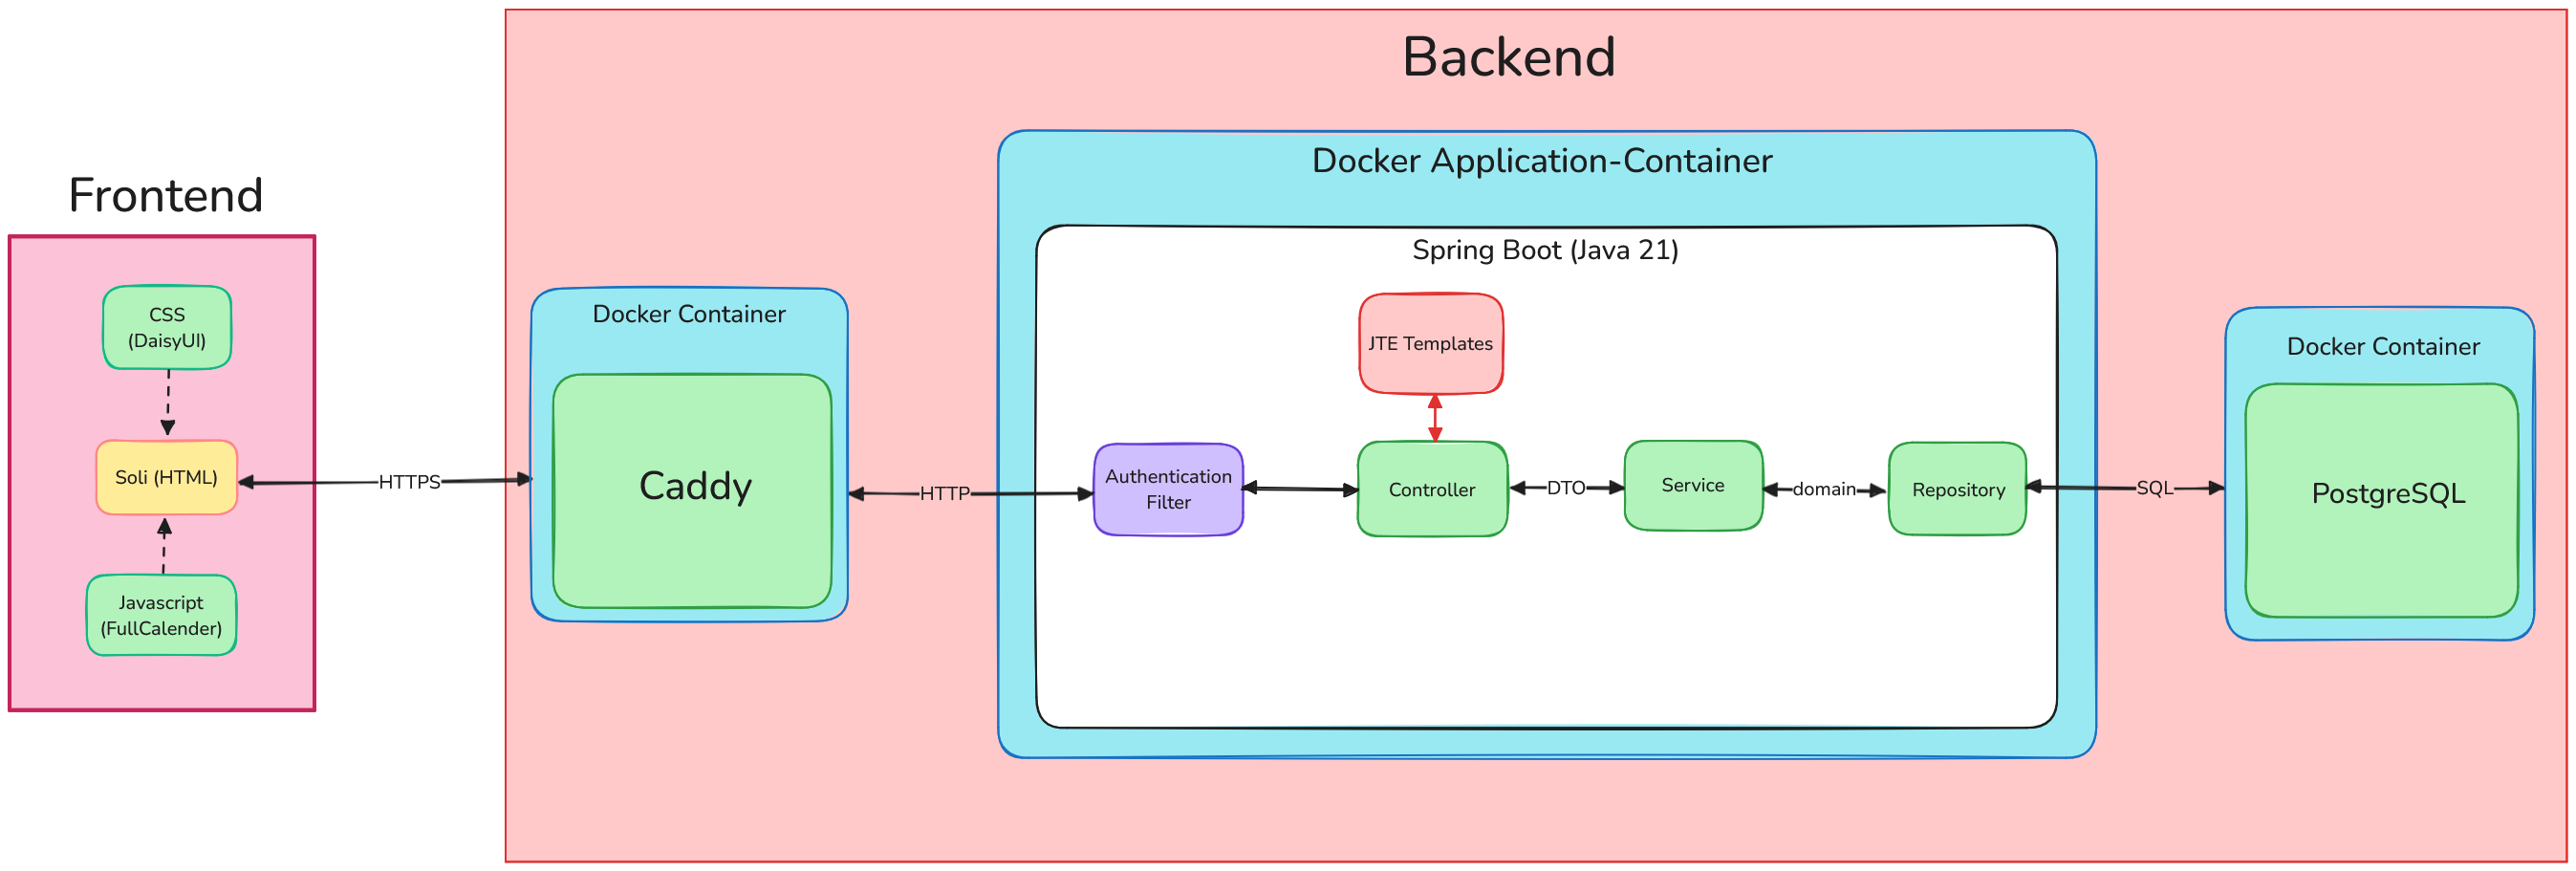
\includegraphics[width=\textwidth]{figures/diagramms/Architekturmodell}
    \label{fig:architekturmodell}
\end{figure}
Die Architektur ist in \textbf{Frontend} und \textbf{Backend} unterteilt und folgt der \textbf{MVC-Struktur} zur klaren Trennung der Verantwortlichkeitsbereiche.
Das \textbf{Frontend} nutzt \textbf{HTML (Soli)}, \textbf{DaisyUI} für das Design und \textbf{FullCalendar} in JavaScript für die Kalenderfunktionalität.
Die Kommunikation mit dem Backend erfolgt sicher über \textbf{HTTPS}.

Ein \textbf{Caddy-Server}, in einem Docker-Container, dient als HTTPS-Reverse-Proxy und leitet Anfragen an das Backend weiter.
Das \textbf{Backend} basiert auf \textbf{Spring Boot} (Java 21) und läuft in einem Docker-Container. Dort prüft ein \textbf{Authentication Filter} die Anfragen,
die von \textbf{Controllern} verarbeitet werden. Mithilfe von \textbf{JTE Templates} werden dynamische HTML-Antworten generiert.
Die \textbf{Businesslogik} liegt in den \textbf{Services}, die Anfragen koordinieren und weiterleiten.
Die \textbf{Repositories} kapseln den SQL-Zugriff und ermöglichen eine saubere, abstrahierte Kommunikation mit der \textbf{PostgreSQL-Datenbank} in einem separaten Container.

Dank \textbf{Server-Side Rendering} bietet die Architektur dynamische Inhalte und hohe Skalierbarkeit. Der Einsatz gängiger Technologien wie \textbf{Docker} sorgt für einfache Bereitstellung und Wartbarkeit.
\clearpage

\section{Klassendiagramm}
\begin{figure}[ht]
    \centering
    \includegraphics[width=0.62\textwidth]{figures/diagramms/klassendiagramm}
    \label{fig:klassendiagramm}
\end{figure}
\clearpage
%!TEX root = ../main.tex

\chapter{Klassenbeschreibung}
\label{ch:class_description}

\todo{Describe all public aspects of the classes, maybe use smaller Klassendiagramme als Hilfe}
%!TEX root = ../main.tex

\chapter{Tests}
\label{ch:tests}

\unsure{do we need Tests?}
\todo{Beschreibungen von Tests welche für die public methods gebraucht werden.} % ????
%!TEX root = ../main.tex

\chapter{Entwurfsmuster}
\label{ch:design_patterns}

\unsure{do we need design patterns?}
\todo{Entwurfsmuster finden und hier beschreiben.} % ????
%!TEX root = ../main.tex

\chapter{Daten}
\label{ch:data}

\todo{Die Datenbank und das Datenbankmodell beschreiben (auch ER modelle nutzen)} % Datenbank (-modell)
%!TEX root = ../main.tex

\chapter{Abläufe}
\label{ch:processes}

\todo{Wichtige und koplexe programmabläufe hier beschreiben. (auch mit sequenz/struktur diagrammen)}

\printglossaries

%------Ende des Dokumentes------------------------------------------------------
\end{document}
